
\documentclass[12pt]{article}
\usepackage{fontspec}
\usepackage[top=0.75in,left=0.8in,right=0.8in,bottom=0.75in]{geometry}
 
%\setmainfont{Times New Roman}
%This would work on a standard latex installation, (your local computer) 
%-----------------------------------------------------------------------
\setromanfont{Phosphate}
\setsansfont{Souvenir}
\setmonofont{Baldur}
%\setromanfont{}
%\setsansfont{}
%\setmonofont[Color={0019D4}]{}
%-----------------------------------------------------------------------

\title{Welcome to Maryn} 
\author{An Introduction to the Table and World} 
\date{As Developed By GLORIOUSSEGFAULT}

\begin{document}
\maketitle

\textsf{D\&D is a form of communal story telling where a bunch of nerds (we, the players) sit around a table and act out heroic (or villainous) deeds as characters in a fantastical world. As the Dungeon Master, my job is to develop and present the world to the players through narration, adjudication, and role playing. As the players, you all have one major job: interact with the world in awesome, magical ways that are character appropriate. This document's purpose is to concisely explain the roles of DM and player as well as the table rules that we should follow during our gaming sessions. Finally, a brief introduction to the world, Maryn, will hopefully pique your interest and inspire character development for the oncoming game.}

\section{The Roles}
\subsection*{The DM}
\paragraph{\textsf{Narration}}
\textsf{As the DM, it is one of my jobs to concisely narrate the environment (people, surroundings) and the zeitgeist (social climate, culture) that the characters find themselves in. The big, bad evil guy/gal (BBEG) should (of course) be evil but also intelligent and complex. The surrounding environment of an encounter is the source of many treasures such as the solution to a riddle, evidence of traps to be disarmed, or the tactical advantage necessary to outmaneuver or overpower the opponent. Cities new to the players are teaming with helpful shopkeepers, conniving thieves, and snooty nobles. Efficient narration brings the environment into focus and inspires the characters into action.}

\textsf{A note to the players: not every described item, detailed hovel, or role-played nonplayer character (NPC) is a plot hook. Red herrings abound in the real world, and so they abound in Maryn as well. Also, the narrator (aka me) is not always to be trusted (see below as well). NPCs are not always telling the truth. Doors are sometimes hidden from view. So, explore the environment and let the DM narrate!}

\paragraph{\textsf{Adjudication}}
\textsf{Another mantle donned by the DM is that of the referee for ``reality'' in the magical world of Maryn. After sufficient narration, the players will decide to take action. Maybe they will attempt to steal the precious MacGuffin out from under the BBEG's nose. It is the DM's job to inform the players what dice rolls are needed to decide the outcome (a stealth check and/or a sleight of hand check) and to silently set the difficulty class (DC) that the characters need to overcome to succeed. If the characters fail at any point during their plan, they might be thrown directly into combat with the BBEG and their minions. At this point, the DM not only guides combat along for the players but also acts for the opponents. Similar duties are required of the DM during noncombat encounters, shopping/crafting days, and downtime.} 

\textsf{As mentioned above, the DM cannot always be trusted. Being human, I will eventually forget a rule or two. Be patient with me. Help me by knowing the rules associated with your character. If evidence for a contended ruling is not readily available, the DM will make a quick decision as to the outcome and look up the rule after the game. Try not to argue about rules but do let me know if I've screwed something up.}

\paragraph{\textsf{Role Playing}}
\textsf{Rather than playing as a single adventurer, the DM is responsible for the portrayal of all NPCs that the characters might encounter during their adventures, from common folk to deities and intelligent villains to wild animals. To truly bring a semblance of life to these roles, I must have an understanding of the desires, fears, alliances, etc for each NPC as well as their mannerisms and mood. This is simple for the wild boar being hunted by the adventuring party but becomes quite time consuming when creating a compelling BBEG, fleshing out the clergy of the Sun God, or developing the various townsfolk that bring a city to life. Please respect this time commitment.} 

\subsection*{The Player}
\paragraph{\textsf{Interaction}}
\textsf{No matter how much time I spend developing Maryn, the world is incomplete and lacking focus without player characters (PCs). Through the actions of the PCs, the players in a D\&D game implicitly take active roles in the development of the world presented by the DM. A good metaphor: the DM prepares a sandbox, filled with sand and toys. The players build an awesome sand castle.} 

\textsf{Using their imagination, the player develops a character's appearance, personality, and backstory as well as decides how the character will react to their surrounding environment. Though these details and interactions may seem unimportant relative to a whole world, don't forget that this particular world has been developed for your character to explore and influence. So, go out and make your character the stuff of legend!}

\paragraph{\textsf{A Brief Note on Backstory Details}}
\textsf{Through the development of their character's backstory, the player can begin to affect the world of Maryn even before the first session of gameplay. Why did their PC decide to become an adventurer? What connections does the character have with their surroundings? Both the DM and players will use the PCs' backgrounds to drive the narrative. Additionally, a fleshed out backstory will affect the character's inherent abilities. Develop the foundation of your character's backstory before the first session. As mentioned below, the more details about the backstory, the better! Use me as a wall to bounce ideas off of when developing your PC's compelling history. At the very least, inform me of your character's background so that I can develop character specific encounters for you.}

\paragraph{\textsf{Awesome is in the Details.}}
\textsf{Which sentence below is more entertaining? \begin{center}``The fighter attacked with his sword, killing the dragon.''\\ or\\ ``With a cry of desperation, the fighter wildly lunged forward with his longsword, slaying the mighty red dragon.''\end{center} The latter is obviously more engaging. This heavy-handed example demonstrates how details add depth to a story. Creative solutions and bold actions are elusive when details are lacking. Therefore, be as explicit as (reasonably) possible when describing the actions taken by your character. Adding exciting details not only enhances the narrative but it could affect the DM's adjudication (see the ``Rule of Cool'' in the next section).}

\textsf{Additionally, players can add depth to their character and the story through role playing. Does your character begin to slur their words while getting drunk at the Feed and Mead Bar and Inn? Can you match your facial expressions with your character's as a bard begins to exaggerate the adventuring party's heroic deeds? What hand motions do you make while casting the spell to call lightning down on your enemies? Peppering such details into gameplay will add reality to the fantastical, unbelievable world of Maryn. Don't forget: role play at your own comfort level.}

\section{Table Rules}
\paragraph{Everyone should enjoy playing in this D\&D campaign.} \textsf{Hands down, this is the most important rule. All other rules in this document and the core rule books are developed with this (\textit{The}) rule in mind. If there is ever a time where you or a set of players are not enjoying the game, then communicate your concerns with the appropriate parties. Note: this rule applies to the DM just as much as it applies to the players. DM burnout is a thing. Players, please be aware of how you are affecting the DM's enjoyment of playing D\&D. DM, perform your duties so as to optimize everyone's enjoyment at the table.} 

\paragraph{The Rule of Cool.}
\textsf{Some of most memorable and fun moments of D\&D are when the PCs perform some extraordinary action that is \textit{almost} unbelievable. More often than not, such moments can only occur when the rules as written (RAW) in the core rule books are bent or interpreted in new, interesting ways. The Rule of Cool specifically allows the players to attempt to reinterpret RAW and make something awesome happen. It is then the DM's job to adjudicate this new and cool thing. Altering RAW for the sake of coolness might increase the DC of an action, thereby making this action more difficult to perform but the results more awesome. Players, recognize that the Rule of Cool should only be used in climactic situations.}

\paragraph{Communication is key.} 
\textsf{Whether you are describing the surroundings or your PC's actions, be detailed in your communication. Generally, leave as little information as possible to be guessed by the other players. This is true for other aspects of the game as well. Please keep the gaming group apprised of scheduling issues or emergency absences. If you have a complaint, issue, or comment for the DM or other player(s), please maturely communicate these issues with the appropriate people. Kicking, screaming, and/or talking behind backs will ruin everyone's fun.}

\paragraph{Sensitive Topics and Themes.}
\textsf{D\&D campaigns are set in fantastical worlds that often have dark, medieval undertones. As the DM, I will do my best to prevent certain undertones from entering our D\&D game. Specifically, torture, graphic or mass death, harm to children, and various forms of abuse will be avoided as best as possible due to their potential for upsetting players. I never want to put one of my players in a situation where they no longer feel comfortable at the gaming table. I, as the DM, am not comfortable with role playing sexual abuse or overly graphic torture/violence. If you are looking for a game that includes these themes, then the game I run is not for you. If there are other themes that you would like me to avoid, please let me know in whatever way you feel comfortable.}

\textsf{If the party finds itself in an encounter that begins to verge on the above topics, I expect everyone at the table to remain mature and respectful. Do not demean or play down the gravity of the situation. If the tone of the campaign is about to shift (e.g. at the start of a new story arc), I will mention any potential for disturbing events/narrative with the players. If the campaign tone is on the tragic side, it is both the DM's and players' jobs to bring the light (aka joviality and hope) to contrast the darkness of the story arc.}

\paragraph{Other rules:} 
\begin{enumerate}
\item\textsf{There will be limited to no ret-conning. Once you've stated what your PC (or NPC) is doing, you cannot take back that action and do something completely different instead. Generally, if dice have been rolled, then the outcome is set in stone.}
\item\textsf{Well thought out planning is important. Attempt to plan \textit{before} the party starts an encounter. Extended strategizing mid-encounter is punishable by loss of actions.}
\item\textsf{Keep meta-gaming to a minimum. If your character remains at the entrance of the cave, then you are unaware of the goblins attacking your compatriots who traveled further below.}
\item\textsf{When interacting with NPCs, assume that they hear whatever you say. For example, the party is trying to swindle a local shopkeep. Any comments made at the table about the attempted swindling will pique the shopkeep's interest and make any deception checks against the poor, small business owner more difficult. The DM assumes that the players are role playing, even if they are not.}
\item\textsf{No backseat DM'ing.}
\item\textsf{Keep an up-to-date character sheet. This includes inventory and money.}
\item\textsf{Practice good table etiquette. Minimize extraneous dice rolls. Don't build dice towers/pyramids. Cell phones should be on silent and away. No messy eating/drink at the table. Please, share food and drink with the DM. }
\item\textsf{If not all players, then at least one player should always take notes during the gaming sessions. A body of notes on the history of the world, backstory details, and supplementary information will be invaluable at some point during the campaign.}
\item\textsf{Any homebrew material introduced or developed by players/DM and agreed upon by the DM is open to modification for gameplay optimization.}
\end{enumerate}

%\paragraph{Gameplay stuff:} 
%\begin{enumerate}
%\item\textsf{PC experience will be narrative based. Rather than earning some numerical value of experience points at the end of each session, the DM will decide that the party has succeed in gaining a level (often after completing a story arch).}
%\item\textsf{Natural 1s and 20s on skill checks do not necessarily correspond to auto-fails or successes, respectively. Rather, Nat 1s or 20s will be used as narrative failures or successes. DCs for skill checks range from 1 (ex: tieing your shoes) to 40+ (ex: free climbing the smooth face of a wall). If you roll a Nat 1 while tieing your shoes, you finally finish putting your shoes on only after minutes of untieing accidental knots made during your attempt. Rolling a Nat 20 on a athletics check to scale the smooth face of a 20 ft wall does not ensure that your character succeeds. If you fail the athletics check even with the Nat 20, then your character might climb about 10 ft before realizing the feutility of the endeavor and gracefully dismounts, landing in superhero pose. Taking 10s and taking 20s on skill checks are allowed, at the cost of in-game time.}
%\end{enumerate}

\section{Maryn, the World}
\textsf{The world of Maryn is a diverse setting that is inhabited by extraordinary magicians, ferocious warriors, stealthy rogues, and devout clerics. The foundations of the present-day civilizations are built on the ruins of ancient predecessors, whose histories have been lost to the sands of time. The future holds exciting potential for both sides in the fight of good versus evil. The pantheon of deities is diverse in style and methods: some gods have massive followings with militarized clergy while other deities chose single champions to forward their goals. The wildernesses and cities alike hold mysteries to be solved, monsters to be slain, and marvels to be ... catalogued. (Damn my failing vocabulary!)}

\textsf{Hopefully, the world that I have described above is an enticing setting to play D\&D within. From my point of view, the current state of Maryn is a shell of what it will become once a group of PCs band together to go adventuring. But, before we begin playing, I leave it up to you, the players, to decide where in Maryn you would like the campaign to be set. Therefore, in this last section, I provide the world map as well as a few notes about the people, cultures, and themes to be found in each major geographical region. Hopefully, these less vague details will sway you when deciding the campaign setting as well as certain details about your character's backstory.}

\begin{figure}[!h]
\begin{center}
\makebox[\textwidth]{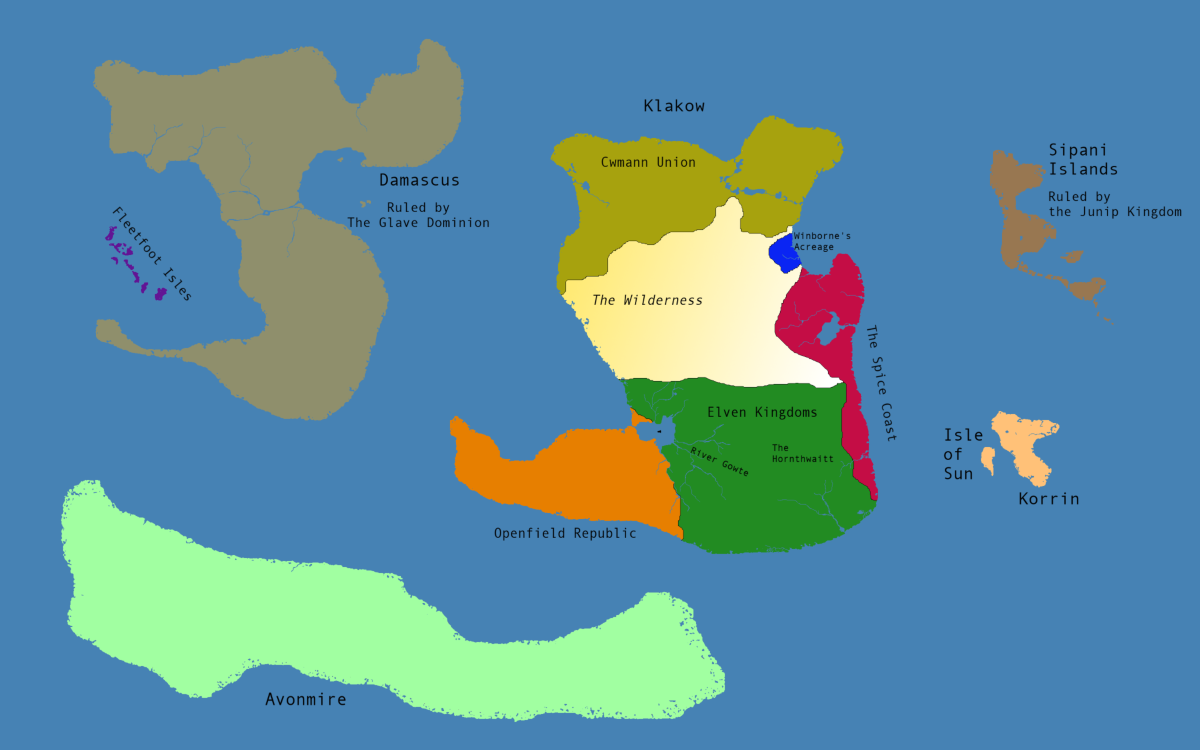
\includegraphics[width=0.95\paperwidth]{world_map_v6.pdf}}
\end{center}
\label{fig:world_map}
\end{figure}

\subsection*{\texttt{Damascus, Ruled by The Glave Dominion}} 
\textsf{The Glave Dominion is an oligarchy that rules the continent of Damascus. The governing body and major industrial centers are located in the central region of the continent. While the Dominion lays claim to the full continent, the northern and southern peninsulas are often neglected by the powers that be. That is, until a revolution or civil disturbance springs to life in these ``less civilized'' regions. Major themes of a campaign set in the Glave Dominion would be oppression and various types of inequality. The PCs will have the opportunity to be the wind that fuels the fire of rebellion \textit{or} the water that quenches it. It is up to you to decide!}

%\textsf{Damascus is the western most continent in Maryn. The southwestern peninsula as well as southern region of the continent is mountainous with high volcanic activity. Central Damascus is mainly coniferous forest and plains. The northern teretories are mainly deciduous forests, eventually giving way to frigid tundras.}
%
%\paragraph{\texttt{The Glave Dominion}}
%\textsf{The Glave Dominion is an oligarchy that rules the continent of Damascus. The governing body and major industrial centers are located in the central region of the continent. While the Dominion lays claim to the full continent, the northern and southern peninsulas are often neglected by the powers that be. That is, until a revolution or civil disturbance springs to life in the ``less civilized'' regions. Major themes of a campaign set in the Glave Dominion would be oppression and various types of inequality. The PCs will have the oppertunity to be the wind that fuels the fire of revolution \textit{or} the water that quenches it. It is up to you to decide!}

\subsection*{\texttt{The Fleetfoot Isles}} 
\textsf{As the name suggests, the Fleetfoot Isles are home to a deft and sly people who make a living off of smuggling people and illicit goods into and out of the Glave Dominion. As long as these activities remain under the radar, the Dominion cares little. PCs originating from these isles will run product into and out of the mainland, using deception and stealth to skirt the Dominion's attention. Characters with a moral compass may find themselves supplying the very same rebellion mentioned above.}

\subsection*{\texttt{Klakow}} 
\textsf{Unlike Damascus, the continent of Klakow is divided into numerous regions due to geography and governments (or lack thereof). Furthering the differences between the two continents, the nation states that pepper this continent are less oppressive against their peoples, thus revolution is not on the menu for PCs living in Klakow. Rather, a focus of campaigns set on this continent will be uncovering the wondrous history of past civilizations, deities, and wildlife. Beyond the gathering of powerful knowledge, adventurers will also have the opportunity to become legendary monster hunters, travel to other planes of reality, commune with the gods, and/or stake their claim to a corner of the continent.}

\paragraph{\texttt{The Cwmann Union}} 
\textsf{The northern territories of Klakow are the motherland of all dwarves. Nearing six centuries ago, the dwarven tribes agreed to aid each other in times of need, thus forming the Cwmann Union. Where once there were ten such tribes, only seven remain. More recently, this alliance has become even more strained due increasingly dire situations: the Sulamit desert encroaches from the south at a seemingly unnatural pace; ancient enemies from the depths below have become more bold; trade with the Glave Dominion has sputtered to a halt due to unknown reasons; traditional dwarven greed has mutated into insatiable lust for riches. Such is dwarven luck! A campaign set within the Cwmann Union will see PCs tackling a subset of these problems in attempts to strengthen the Union's foundation. Additionally, the PCs will have the potential to build their very own stronghold, becoming the eighth beacon of hope in the north.}

\paragraph{\texttt{The Openfield Republic}} 
\textsf{The southwestern peninsula of Klakow is home to the people of the Openfield Republic. Founded on the principle of religious freedom, the Republic is ruled by representative clergy members from each major faith. Yet, in this land of holiness and acceptance, extremists of faith are abundant and clashes between the faithful have eroded at the Republic's foundation. Furthermore, in certain shadowy corners of the Republic, followers of dark and dangerous gods take advantage of the government's principles to further their evil plans. As a campaign setting, the Openfield Republic will provide ample opportunities for the PCs to demonstrate their faith (or lack there of) in the gods.}

\paragraph{\texttt{The Spice Coast}} 
\textsf{Klakow is home to rare, powerful, and misunderstood resources. The colonies of the Spice Coast are the world's black market, where the plundered goods from the continent are traded with little impunity. Rather than a unified government, each port city is controlled by a respective trading company with their own laws, militia, and economies. Beyond the aggressive competition for assets, peace is maintained between the cities for the sake of profit. Do certain companies have an ulterior motive for the aggressive pillaging of the wildernesses? Guided by their morals or the prospect of a payday, PCs will explore the exotic environments of cities and wilderness alike, gathering reputation or respect, wealth or allies. Through various avenues, the players will have the opportunity to develop their own economic dynasty.}

\paragraph{\texttt{The Elven Kingdoms, The Wilderness of Klakow, Winborne's Acreage}} 
\textsf{These regions of Klakow are not viable starting points for a campaign. Rather, these regions will open up as the PCs garner strength and allies.}

\subsection*{\texttt{Avonmire}} 
\textsf{Avonmire is extreme in all facets. Thin coniferous forests speckle the northern shores while all else can simply be described as tundra and icy plateau. In such an inhospitable environment, only the strong survive and so Avonmire is the home to hardened nomadic tribes. While an outsider would only see a brutish and uncivilized people, a deep history and culture underlies these people. The main theme in a campaign set in Avonmire is survival, pure and simple. The wild beasts of the frigid environment are both threats and food sources (as well as chances to prove your bravery). Slaving ships from Damascus lure or kidnap young and capable heads away to warmer climes. The smallest slight against another tribe will lead to war. On a brighter note, ``spring'' on the northern shore is said to be exceptionally beautiful, so the continent has that going for it. Similar to campaign settings in Klakow, PCs will have the opportunity to earn the trust of followers and build their own stronghold, specifically a nomadic barbarian tribe in this setting.}

\subsection*{\texttt{The Junip Kingdom}} 
\textsf{Fabled as the home of all dragon-kind, the Sipani island chain is now controlled by the Junip Kingdom. The dragonborn people are proud and innately powerful, with a mistrust of outsiders. Beyond the kingdom, these scaled humanoids are rare, awesome, and hunted. Further details of a campaign starting in the Junip Kingdom will depend on the characters to be played but certain themes will be common: abduction, theft, and ancient dragons.}

\subsection*{\texttt{The Isles of Korrin and Sun}} 
\textsf{An archeology team has recently landed on the abandoned island of Korrin. Ancient magics and incorporeal threats left behind from a civilization lost to history lie in store for the group. Alien languages, deteriorating traps, and dangerous inhabitants will be just a few of the obstacles to be overcome as the PCs attempt to complete their dig. As a setting, the islands of Korrin and Sun are most analogous to classic dungeon delving adventures. Through astute exploration of the islands, PCs will uncover forgotten theories defining the magics present in the world of Maryn. Additionally, delving ever deeper into the ruined civilization may lure the PCs into direct confrontation with ancient deities, monsters, and/or constructs. Happy digging!}

\end{document}
% Baldur.ttf, Convergence-Regular.ttf, Souvenir.ttf, Phosphate.ttc

